\documentclass[tikz,border=5mm]{standalone}
\usetikzlibrary{decorations.markings}

\begin{document}
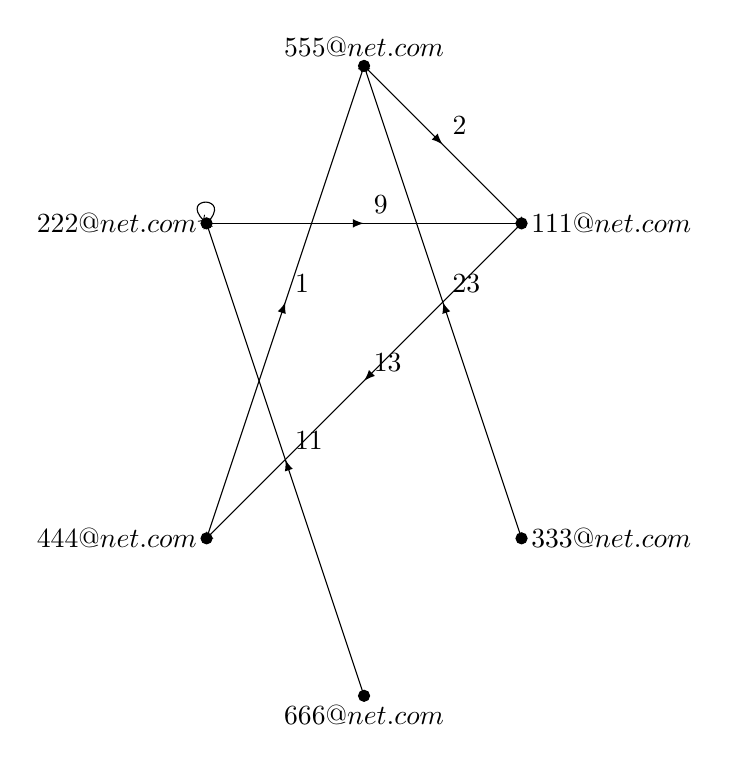
\begin{tikzpicture}
    \tikzset{
        myarrow/.style={
            postaction={
                decorate,
                decoration={
                    markings,
                    mark=at position #1 with {\arrow{latex}},
                },
            },
        },
    }

    % Vertices
    \draw[fill=black] (4, 4) circle (2pt) node[right] {$111@net.com$};
    \draw[fill=black] (0, 4) circle (2pt) node[left] {$222@net.com$};
    \draw[fill=black] (4, 0) circle (2pt) node[right] {$333@net.com$};
    \draw[fill=black] (0, 0) circle (2pt) node[left] {$444@net.com$};
    \draw[fill=black] (2, 6) circle (2pt) node[above] {$555@net.com$};
    \draw[fill=black] (2, -2) circle (2pt) node[below] {$666@net.com$};

    % Arcs
    \draw[->, myarrow=.5] (2,6) -- node[midway, above right] {2}  (4,4);
    \draw[->, myarrow=.5] (4,4) -- node[midway, above right] {13}  (0,0);
    \draw[->, myarrow=.5] (4,0) -- node[midway, above right] {23}  (2,6);
    \draw[->, myarrow=.5] (0,0) -- node[midway, above right] {1}  (2,6);
    \draw[->, myarrow=.5] (2,-2) -- node[midway, above right] {11}  (0,4);
    \draw[->, myarrow=.5] (0,4) -- node[midway, above right] {9}  (4,4);

    \path[every node/.style={font=\sffamily\small}]
    (0,4)   edge[loop] node  {} (0);
\end{tikzpicture}
\end{document}
